\documentclass[12pt, notitlepage, final]{article} 

\newcommand{\name}{Vince Coghlan}

%\usepackage[dvips]{graphics,color}
\usepackage{amsfonts}
\usepackage{amssymb}
\usepackage{amsmath}
\usepackage{latexsym}
\usepackage{enumerate}
\usepackage{amsthm}
\usepackage{nccmath}
\usepackage{setspace}
\usepackage[pdftex]{graphicx}
\usepackage{epstopdf}
\usepackage[siunitx]{circuitikz}
\usepackage{tikz}
\usepackage{float}
\usepackage{cancel} 
\usepackage{setspace}
\usepackage{overpic}
\usepackage{mathtools}
\usepackage{listings}
\usepackage{color}
\usepackage{qtree}
%\usepackage{gensymb}

\usetikzlibrary{calc}
\usetikzlibrary{matrix}
\usetikzlibrary{positioning}

\numberwithin{equation}{section}
\DeclareRobustCommand{\beginProtected}[1]{\begin{#1}}
\DeclareRobustCommand{\endProtected}[1]{\end{#1}}
\newcommand{\dbr}[1]{d_{\mbox{#1BR}}}
\newtheorem{lemma}{Lemma}
\newtheorem*{corollary}{Corollary}
\newtheorem{theorem}{Theorem}
\newtheorem{proposition}{Proposition}
\theoremstyle{definition}
\newtheorem{define}{Definition}
\newcommand{\column}[2]{
\left( \begin{array}{ccc}
#1 \\
#2
\end{array} \right)}

\newdimen\digitwidth
\settowidth\digitwidth{0}
\def~{\hspace{\digitwidth}}

\setlength{\parskip}{1pc}
\setlength{\parindent}{0pt}
\setlength{\topmargin}{-3pc}
\setlength{\textheight}{9.0in}
\setlength{\oddsidemargin}{0pc}
\setlength{\evensidemargin}{0pc}
\setlength{\textwidth}{6.5in}
\newcommand{\answer}[1]{\newpage\noindent\framebox{\vbox{{\bf ECEN 5018 Spring 2014} 
\hfill {\bf \name} \vspace{-1cm}
\begin{center}{Homework \#5}\end{center} } }\bigskip }

\DeclareMathOperator*{\argmin}{arg\,min}

%absolute value code
\DeclarePairedDelimiter\abs{\lvert}{\rvert}%
\DeclarePairedDelimiter\norm{\lVert}{\rVert}
\makeatletter
\let\oldabs\abs
\def\abs{\@ifstar{\oldabs}{\oldabs*}}
%
\let\oldnorm\norm
\def\norm{\@ifstar{\oldnorm}{\oldnorm*}}
\makeatother

\def\dbar{{\mathchar'26\mkern-12mu d}}
\def \Frac{\displaystyle\frac}
\def \Sum{\displaystyle\sum}
\def \Int{\displaystyle\int}
\def \Prod{\displaystyle\prod}
%\def \P[x]{\Frac{\partial}{\partial x}}
%\def \D[x]{\Frac{d}{dx}}
\newcommand{\PD}[2]{\frac{\partial#1}{\partial#2}}
\newcommand{\PF}[1]{\frac{\partial}{\partial#1}}
\newcommand{\DD}[2]{\frac{d#1}{d#2}}
\newcommand{\DF}[1]{\frac{d}{d#1}}
\newcommand{\fix}[2]{\left(#1\right)_#2}
\newcommand{\ket}[1]{|#1\rangle}
\newcommand{\bra}[1]{\langle#1|}
\newcommand{\braket}[2]{\langle #1 | #2 \rangle}
\newcommand{\bopk}[3]{\langle #1 | #2 | #3 \rangle}
\newcommand{\Choose}[2]{\displaystyle {#1 \choose #2}}
\newcommand{\proj}[1]{\ket{#1}\bra{#1}}
\def\del{\vec{\nabla}}
\newcommand{\avg}[1]{\langle#1\rangle}
\newcommand{\piecewise}[4]{\left\{\beginProtected{array}{rl}#1&:#2\\#3&:#4\endProtected{array}\right.}
\newcommand{\systeme}[2]{\left\{\beginProtected{array}{rl}#1\\#2\endProtected{array}\right.}
\def \KE{K\!E}
\def\Godel{G$\ddot{\mbox{o}}$del}

%\onehalfspacing

\begin{document}

\answer{}

\textbf{1)} Consider the following cost sharing problem:
\begin{itemize}
  \item{Player set: $N=\{1,2,3\}$}
  \item{Opportunity costs: $c:2^N \rightarrow R$}
\end{itemize}
\[
  c(\{1\})=9\text{,  }\hspace{3mm}c(\{2\})=8\text{,  }\hspace{3mm}c(\{3\})=9
\]
\[
  c(\{1,2\})=14\text{,  }c(\{1,3\})=15\text{,  }c(\{2,3\})=13
\]
\[
  c(\{1,2,3\})=20\hspace{3cm}c(\{\emptyset\})=0\hspace{1cm}
\]

\begin{enumerate}[(a)]
  \item{Identify the core graphically}\\
    \begin{figure}[H]
    \begin{center}
    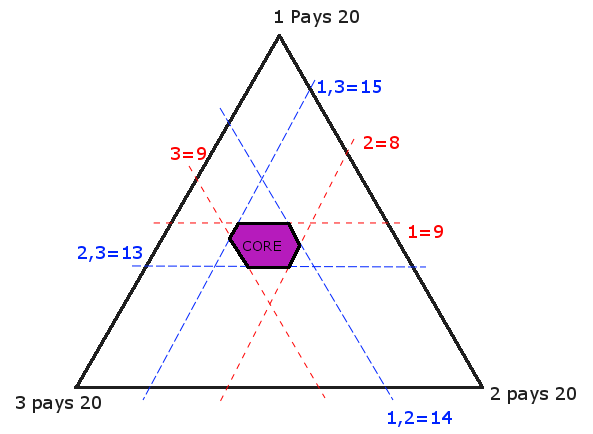
\includegraphics[width=9cm]{f1}
    \end{center}
    \end{figure}
  \item{Is the core nonempty?}\\
    Yes, as can be seen in the picture.
  \item{Compute the marginal contribution for each player.}\\
    The marginal cost of each player will be the marginal cost to the full coalition, for
    player 1:
    \[
      c(\{1,2,3\})-c(\{2,3\}) = 7
    \]
    for player 2:
    \[
      c(\{1,2,3\})-c(\{1,3\}) = 5
    \]
    and player 3:
    \[
      c(\{1,2,3\})-c(\{1,2\}) = 6
    \]
  \item{Compute the Shapley value for each player using equation in notes}\\
    The equation in the notes is:
    \[
      Sh(i,S;c)=\sum_{T\subseteq S\backslash\{i\}} \frac{|T|!(|S|-|T|-1)!}{|S|!}(c(T\cup\{i\})-c(T))
    \]
    For player 1:
    \[
      Sh(1,\{1,2,3\};c)=\frac{2}{6}(c(\{1,2,3\})-c(\{2,3\})) + \frac{1}{6}(c(\{1,2\})-c(\{2\})) + 
    \]
    \[
      \frac{1}{6}(c(\{1,3\})-c(\{3\})) + \frac{2}{6}(c(\{1\})-c(\{\emptyset\})) = 7\frac{1}{3}
    \]
    For player 2:
    \[
      Sh(2,\{1,2,3\};c)=\frac{2}{6}(c(\{1,2,3\})-c(\{1,3\})) + \frac{1}{6}(c(\{1,2\})-c(\{1\})) + 
    \]
    \[
      \frac{1}{6}(c(\{2,3\})-c(\{3\})) + \frac{2}{6}(c(\{2\})-c(\{\emptyset\})) = 5\frac{5}{6}
    \]
    For player 3:
    \[
      Sh(3,\{1,2,3\};c)=\frac{2}{6}(c(\{1,2,3\})-c(\{1,2\})) + \frac{1}{6}(c(\{1,3\})-c(\{1\})) + 
    \]
    \[
      \frac{1}{6}(c(\{2,3\})-c(\{2\})) + \frac{2}{6}(c(\{3\})-c(\{\emptyset\})) = 6\frac{5}{6}
    \]
  \item{Compute the Shapley value for each player using ordering approach in notes}\\
    The marginal contribution over all oderings can be easily calculated from the marginal
    values.  These must be found for each ordering, as seen below:
    \[
      3\leftarrow2\leftarrow1 \Rightarrow c(\{1,2,3\}) - c(\{2,3\}) = 7
    \]
    \[
      2\leftarrow3\leftarrow1 \Rightarrow c(\{1,2,3\}) - c(\{2,3\}) = 7
    \]
    \[
      2\leftarrow1\leftarrow3 \Rightarrow c(\{1,2\}) - c(\{2\}) = 6
    \]
    \[
      3\leftarrow1\leftarrow2 \Rightarrow c(\{1,3\}) - c(\{3\}) = 6
    \]
    \[
      1\leftarrow3\leftarrow2 \Rightarrow c(\{1\}) - c(\{\emptyset\}) = 9
    \]
    \[
      1\leftarrow2\leftarrow3 \Rightarrow c(\{1\}) - c(\{\emptyset\}) = 9
    \]
    For player 2:
    \[
      3\leftarrow1\leftarrow2 \Rightarrow c(\{1,2,3\}) - c(\{1,3\}) = 5
    \]
    \[
      1\leftarrow3\leftarrow2 \Rightarrow c(\{1,2,3\}) - c(\{1,3\}) = 5
    \]
    \[
      3\leftarrow2\leftarrow1 \Rightarrow c(\{2,3\}) - c(\{3\}) = 4
    \]
    \[
      1\leftarrow2\leftarrow3 \Rightarrow c(\{1,2\}) - c(\{1\}) = 5
    \]
    \[
      2\leftarrow3\leftarrow1 \Rightarrow c(\{2\}) - c(\{\emptyset\}) = 8
    \]
    \[
      2\leftarrow1\leftarrow3 \Rightarrow c(\{2\}) - c(\{\emptyset\}) = 8
    \]
    For player 3:
    \[
      2\leftarrow1\leftarrow3 \Rightarrow c(\{1,2,3\}) - c(\{1,2\}) = 6
    \]
    \[
      1\leftarrow2\leftarrow3 \Rightarrow c(\{1,2,3\}) - c(\{1,2\}) = 6
    \]
    \[
      2\leftarrow3\leftarrow1 \Rightarrow c(\{2,3\}) - c(\{2\}) = 5
    \]
    \[
      1\leftarrow3\leftarrow2 \Rightarrow c(\{1,3\}) - c(\{1\}) = 6
    \]
    \[
      3\leftarrow2\leftarrow1 \Rightarrow c(\{3\}) - c(\{\emptyset\}) = 9
    \]
    \[
      3\leftarrow1\leftarrow2 \Rightarrow c(\{3\}) - c(\{\emptyset\}) = 9
    \]
    We can then calculate the shapley value for each player, for player 1:
    \[
      \frac{1}{6}(7+7+6+6+9+9) = 7\frac{1}{3}
    \]
    for player 2:
    \[
      \frac{1}{6}(5+5+4+5+8+8) = 5\frac{5}{6}
    \]
    for player 3:
    \[
      \frac{1}{6}(6+6+5+6+9+9) = 6\frac{5}{6}
    \]
    Note that when we add these together we get 20.
  \item{Verify approaches in (d) and (e) result in the same answer.}\\
    Yes it is.
\end{enumerate}


\textbf{2)} Consider the following social choice problem with externalities:
\begin{itemize}
  \item{Three bidders $\{x,y,z\}$}
  \item{Three possible allocations $\{X,Y,Z\}$ where $X$ indicates object givin $x$}
  \item{Player specific valuations of allocations:}
    \begin{center}
      \begin{tabular}{c | c | c | c |}
        \multicolumn{4}{c}{\hspace{4mm} $X$ \hspace{2.7mm} $Y$ \hspace{2.7mm} $Z$}\\
        \cline{2-4}
        $x$ & 30 & 0 & -15 \\
        \cline{2-4}
        $y$ & 10 & 40 & 0 \\
        \cline{2-4}
        $z$ & 0 & -10 & 50 \\
        \cline{2-4}
      \end{tabular}
    \end{center}
\end{itemize}
\begin{enumerate}[(a)]
  \item{Discuss the VCG mechanism for this problem.  What allocation is chosen? What prices are charged
    to the players} \\
    The VCG mechanism will make an attempt to make the action of reporting your true value, the dominant
    strategy for any player.  We can see in this particular problem that $x$ would like to win the least,
    but also would like $z$ to lose the most.  $y$ would like to win the second most, but also wants $x$
    to win.  $z$ would like to win the most, but also wants $y$ to lose.  These externalities relate to
    the real life externalities that make designing mechanisms for games so hard.  We will see that the
    VCG mechanism will solve many of our problems.  Each player is going to have to pay a tax related
    to the externalities.  We can find this like so ($\hat{v}$ is the reported value):
    \[
      t_i(\hat{v}) = \sum_{j\neq i}\hat{v}_j(x^*(\hat{v})) - \sum_{j\neq i}\hat{v}_j(x^*(\hat{v}_{-i}))
    \]
    for example:
    \[
      t_1 = 10 \; t_2 = -10 \; t_3 = -15
    \]
    Each bid by each player will be processed through this mechanism.  If we assume each player is to bid
    his value of the item, we can see that the allocation would look like $\{40,30,35\}$ and $x$ would
    win the object.
  \item{Prove that the VCG mechanism is efficient for this problem.} \\
    To prove that this is efficient we must prove two things, first that the game induces the players
    to report truthfully, and second, to provide the utilitarian social choice.  We will start witht the
    first one.  To prove that each player will report truthfully, we will follow closely the general proof
    for this mechanism that is found in the lecture notes.  First, the utility for any player given that
    he bids something $\hat{v}_i$ and that everyone else bids $\hat{v}_{-i}$(remember we want our
    mechanism to provide a dominant strategy regardless of what other players do) is:
    \[
      v_i(x^*(\hat{v}_i,\hat{v}_{-i}))+t_i(\hat{v}_i,\hat{v}_{-i})
    \]
    We can substitute in for $t_i$:
    \[
      v_i(x^*(\hat{v}_i,\hat{v}_{-i})) + \sum_{j\neq i}\hat{v}_j(x^*(\hat{v}_i,\hat{v}_{-i})) - \sum_{j\neq i}\hat{v}_j(x^*(\hat{v}_{-i}))
    \]
    Since player $i$ cannot modify the last term if he is trying to best respond, we will just maximize
    the first two terms:
    \[
      \underset{\hat{v}_i}{\text{arg}\max}\; v_i(x^*(\hat{v}_i,\hat{v}_{-i})) + \sum_{j\neq i}\hat{v}_j(x^*(\hat{v}_i,\hat{v}_{-i}))
    \]
    Player $x$ will want to choose an $x$ such that 

\end{enumerate}

\end{document}
